%%%%%%%%%%%%%%%%%%%%%%%%%%%%%%%%%%%%%%%%%%%%%%%%%%%%%%%%%%%%%%%%%%%%%
%% This is a (brief) model paper using the achemso class
%% The document class accepts keyval options, which should include
%% the target journal and optionally the manuscript type.
%%%%%%%%%%%%%%%%%%%%%%%%%%%%%%%%%%%%%%%%%%%%%%%%%%%%%%%%%%%%%%%%%%%%%
\documentclass[journal=jacsat,manuscript=article]{achemso}

%%%%%%%%%%%%%%%%%%%%%%%%%%%%%%%%%%%%%%%%%%%%%%%%%%%%%%%%%%%%%%%%%%%%%
%% Place any additional packages needed here.  Only include packages
%% which are essential, to avoid problems later. Do NOT use any
%% packages which require e-TeX (for example etoolbox): the e-TeX
%% extensions are not currently available on the ACS conversion
%% servers.
%%%%%%%%%%%%%%%%%%%%%%%%%%%%%%%%%%%%%%%%%%%%%%%%%%%%%%%%%%%%%%%%%%%%%
\usepackage[version=3]{mhchem} % Formula subscripts using \ce{}
\usepackage{color}  % remove this package once you are done
%%%%%%%%%%%%%%%%%%%%%%%%%%%%%%%%%%%%%%%%%%%%%%%%%%%%%%%%%%%%%%%%%%%%%
%% If issues arise when submitting your manuscript, you may want to
%% un-comment the next line.  This provides information on the
%% version of every file you have used.
%%%%%%%%%%%%%%%%%%%%%%%%%%%%%%%%%%%%%%%%%%%%%%%%%%%%%%%%%%%%%%%%%%%%%
%%\listfiles

%%%%%%%%%%%%%%%%%%%%%%%%%%%%%%%%%%%%%%%%%%%%%%%%%%%%%%%%%%%%%%%%%%%%%
%% Place any additional macros here.  Please use \newcommand* where
%% possible, and avoid layout-changing macros (which are not used
%% when typesetting).
%%%%%%%%%%%%%%%%%%%%%%%%%%%%%%%%%%%%%%%%%%%%%%%%%%%%%%%%%%%%%%%%%%%%%
\newcommand*\mycommand[1]{\texttt{\emph{#1}}}
%%%%%%%%%%%%%%%%%%%%%%%%%%%%%%%%%%%%%%%%%%%%%%%%%%%%%%%%%%%%%%%%%%%%%
%% Meta-data block
%% ---------------
%% Each author should be given as a separate \author command.
%%
%% Corresponding authors should have an e-mail given after the author
%% name as an \email command. Phone and fax numbers can be given
%% using \phone and \fax, respectively; this information is optional.
%%
%% The affiliation of authors is given after the authors; each
%% \affiliation command applies to all preceding authors not already
%% assigned an affiliation.
%%t
%% The affiliation takes an option argument for the short name.  This
%% will typically be something like "University of Somewhere".
%%
%% The \altaffiliation macro should be used for new address, etc.
%% On the other hand, \alsoaffiliation is used on a per author basis
%% when authors are associated with multiple institutions.
%%%%%%%%%%%%%%%%%%%%%%%%%%%%%%%%%%%%%%%%%%%%%%%%%%%%%%%%%%%%%%%%%%%%%
\author{Ruchi Lohia}
%\altaffiliation{A shared footnote}
\author{Reza Salari}
%\altaffiliation{Current address: Some other place, Othert\"own,
%Germany}
\author{Grace Brannigan}
\email{grace.brannigan@rutgers.edu(GB)}
\affiliation[Rutgers University]
{Center for Computational and Integrative Biology, Rutgers University, Camden, NJ, USA}
\alsoaffiliation[Rutgers University]
{ Department of Physics, Rutgers University, Camden, NJ, USA}

%%%%%%%%%%%%%%%%%%%%%%%%%%%%%%%%%%%%%%%%%%%%%%%%%%%%%%%%%%%%%%%%%%%%%
%% The document title should be given as usual. Some journals require
%% a running title from the author: this should be supplied as an
%% optional argument to \title.
%%%%%%%%%%%%%%%%%%%%%%%%%%%%%%%%%%%%%%%%%%%%%%%%%%%%%%%%%%%%%%%%%%%%%
\title[An \textsf{achemso} demo]
  {Mechanism underlying conformational effects of the disease-associated Val66Met substitution on the intrinsically disordered region of proBDNF\footnote{A footnote for the title}}

%%%%%%%%%%%%%%%%%%%%%%%%%%%%%%%%%%%%%%%%%%%%%%%%%%%%%%%%%%%%%%%%%%%%%
%% Some journals require a list of abbreviations or keywords to be
%% supplied. These should be set up here, and will be printed after
%% the title and author information, if needed.
%%%%%%%%%%%%%%%%%%%%%%%%%%%%%%%%%%%%%%%%%%%%%%%%%%%%%%%%%%%%%%%%%%%%%
\abbreviations{IR,NMR,UV}
\keywords{American Chemical Society, \LaTeX}
\newcommand{\grace}[1]{\textcolor{blue}{#1}}
\newcommand{\ruchi}[1]{\textcolor{red}{#1}}
\newcommand{\sticky}{proglobular~}
\usepackage{makecell}

\renewcommand\theadalign{bc}
\renewcommand\theadfont{\bfseries}
\renewcommand\theadgape{\Gape[4pt]}
\renewcommand\cellgape{\Gape[4pt]}
\begin{document}
%%%%%%%%%%%%%%%%%%%%%%%%%%%%%%%%%%%%%%%%%%%%%%%%%%%%%%%%%%%%%%%%%%%%%
%% The manuscript does not need to include \maketitle, which is
%% executed automatically.  The document should begin with an
%% abstract, if appropriate.  If one is given and should not be, the
%% contents will be gobbled.
%%%%%%%%%%%%%%%%%%%%%%%%%%%%%%%%%%%%%%%%%%%%%%%%%%%%%%%%%%%%%%%%%%%%%
\begin{abstract}
Although the role of electrostatic interactions and mutations that change charge states in intrinsically disordered proteins (IDPs) is well-established, many disease-associated mutations in IDPs are charge-neutral. The Val66Met mutation encodes a hydrophobic-to-hydrophobic mutation at the midpoint of the prodomain of precursor brain-derived neurotrophic factor (BDNF), one of the earliest mutations to be associated with neuropsychiatric disorders, for which the underlying molecular mechanism is unknown. Here we report on $\sim$ 0.5ms fully-atomistic explicit solvent temperature replica exchange molecular dynamics simulations of the 91 residue prodomain, for both the V66 and M66 sequence with neutral and protonated adjacent histidine.
We show that the highly disordered prodomain can be meaningfully divided into domains based on sequence alone. We find that the tertiary contact preference is determined by individual domains' mean hydrophobicity, net charge and it's distribution. Furthermore, we find the prevalence of Met-Met interactions in M66 sequence, these interactions have been under-appreciated in IDPs. 
The simulations were able to correctly reproduce the location of both local and non-local secondary changes due to the mutation when compared with NMR spectroscopy\cite{Anastasia2013}. We find that the local structure change is mediated via entropic and sequence specific effects. Interestingly, we find that the non-local secondary structure change is not mediated via change in tertiary contact preference but rather it is mediated via change in local secondary structure preference. 
%Long-range tertiary contact between h2b domain and h3a domain is coupled with beta and helicity at either domains in V66 and M66 respectively.
%Protonated histidine increases the formation of long helices and eliminates the beta structure tendency at SNP domain in both V66 and M66 forms. The helix coupling at residue h2b and h3a is in-sensitive to protonation in M66 sequence. However, protonated V66 sequence, looses $\beta$ coupling, probably due to loss of a salt-bridge at E64:R93.
\end{abstract}

%%%%%%%%%%%%%%%%%%%%%%%%%%%%%%%%%%%%%%%%%%%%%%%%%%%%%%%%%%%%%%%%%%%%%
%% Start the main part of the manuscript here.
%%%%%%%%%%%%%%%%%%%%%%%%%%%%%%%%%%%%%%%%%%%%%%%%%%%%%%%%%%%%%%%%%%%%%

\section*{Introduction}

The physiological significance of intrinsically disordered proteins (IDPs), which can explore a wide range of conformational ensembles in their functional form, ~\cite {Uversky2013a,Panchenko2015,Ward2004a,Dyson2005a} is now well-established. More than 33\% of eukaryotic proteins contain disordered regions longer than 30 residues \cite{Ward2004a}, many of which are involved in critical biological functions, including transcriptional regulation and cell signaling \cite{Dunker2005}.  Long intrinsically disordered regions are particularly abundant among cancer and neurodegenerative-associated proteins\cite{Habchi2014,Babu2011}.  

IDP amino-acid sequences tend to be low complexity and include numerous charged residues, often in long repeats ~\cite{Uversky2013a}. In contrast to ordered proteins, in which a complex sequence encodes a well-defined tertiary structure, an IDP sequence determines a heterogeneous conformational ensemble.  More than 35\% of 
IDPs reported in DISPROT ~\cite {Sickmeier2007a} are strong polyampholytes, and their ensemble properties can be predicted using statistical theories of polyampholytes from polymer physics and global properties of the sequence, including the fraction of charged residues and the separation of oppositely charged residues (Fig~\ref{fig1}a)~\cite{Das2015,Das2013a}.  This role is consistent with the long-range nature of electrostatic interactions, which can affect coupling between distant residues in an otherwise disordered structure.  


Although IDP sequences are low-complexity and do not encode a well-defined structure, single residue substitutions can still have functional effects that are significant for the organism.  More than 20\% of disease-associated missense single nucelotide polymorphisms (SNPs) are found in IDPs;\cite{Vacic2012a} although detectable, the relatively subtle functional effects may lead to relatively weak selection pressure, whether positive or negative, allowing the mutation to persist at high frequencies within a population.  Numerous structural and simulation studies ~\cite{Larini2013b,Ganguly2015,Viet2014a,Viet2013,Truong2014a,Zhan2013a,Xu2013a} have demonstrated clear effects of single charged-residue insertion, deletion, or substitutions on conformational ensemble and aggregation of IDPs monomers. Single charged residue mutations or post tranlational modifications that change charges will affect the sequence electrostatics %(such as fraction and separation of charged residues) 
predicted to determine ensemble properties simply from statistical physics models, and in short-chains, can also induce qualitative changes by changing the appropriate regime. ~\cite{Das2015,Larini2013b,Bah2016,He2015}. 
Locally, such mutations can modulate residual secondary structure preferences via forming or breaking local salt-bridges or by introducing helix breaking residues. ~\cite{AlexanderConicella2016,Ganguly2015,Zhan2013a}. Hydrophobicity dependent compaction has been observed in disordered domain of poly(A)-binding protein. ~\cite {Riback2017}.
  
For IDPs with a relatively low fraction of charged residues, typical of the Janus region of the state diagram proposed by Das and Pappu\cite{Das2015,Das2013a} (Fig~\ref{fig1}a), more subtle differences among neutral amino-acids  play an increasingly important role in determining the ensemble.  More than 15\% of disease-associated IDP polymorphisms are substitutions between two charge-neutral residues. ~\cite {Vacic2012a} The extent to which such substitutions in IDPs can affect non-local aspects of the conformational ensemble is uncertain;  such substitution directly affects short-range interactions, and structure-based coupling between distant residues in IDPs is expected to be weak.  Nonetheless, correlations between secondary structure of distant residues has been frequently observed in IDPs ~\cite{Ganguly2015,Iesmantavicius2013}; for example, several cancer mutations in transactivation domain of tumor suppressor p53 can lead to helicity changes in residues sequentially far away from the mutation sites ~\cite{Ganguly2015}.

In structured proteins, contacts between residues distant along the sequence are reflected in the tertiary structure, but developing a framework for describing the analogous property in IDPs has not been straightforward. Among traditional structural biology techniques, NMR has been most useful for characterizing IDPs, but is frequently limited to residual secondary structure (Ref. \cite{Mittag2007,Habchi2014} and references therein). Molecular dynamics (MD) simulations have played a significant role in understanding IDP structure and dynamics ~\cite{Stanley2015,Ithuralde2016,Knott2012b,Invernizzi2013,Abeln2008,Yedvabny2015,Levine2017a}, but face limitations on chain length similar to those incurred in simulations of protein folding; most unbiased simulations have been performed in implicit solvent and/or involve chains too short to meaningfully sample contacts between residues far apart on the peptide chain.  Studies of aggregation among multiple shorter monomeric IDPs ~\cite{Levine2015,Pappu2008}  have provided some of the most useful frameworks for considering tertiary contacts between residues which are distantly connected along the peptide backbone.  Point mutations are also known to affect these contacts via differential salt-bridge and hydrogen-bonding formations, with mutations that change charge states affecting conformational ensemble via altered salt-bridge networks. ~\cite{Levine2015} 

Many mutations in IDPs are associated with neurological, aging-associated neurodegenerative, or psychiatric disorders; despite an exponential increase in the amount of available genetic data, identifying the genetic origins of such disorders has proven remarkably challenging, with few variants identified as replicable predictors of disease.  %despite heritability rates for major disorders reaching 40-70\%.\cite{Alhajji2015} 
One of the earliest identified variants is the Val66Met mutation (rs6265)  in the pro-domain region of Brain-derived Neurotrophic Factor (BDNF), \cite{Notaras2015} a signaling protein %critical for neuronal development and plasticity 
that retains a critical role in neurogenesis and synaptogenesis throughout adulthood(Fig~\ref{fig1}b).\cite{Korte1995} It has been implicated in maintenance of the hippocampus and the mechanism underlying action of numerous antidepressants, \cite{Autry2012,Bjorkholm2016} %(http://www.ncbi.nlm.nih.gov/pmc/articles/PMC3310485/#B15) 
including rapidly acting low-dose ketamine.\cite{Autry2011}  An extensive library of genome-wide association (and even earlier) studies have repeatedly identified the Val66Met mutation as reducing hippocampal volume and episodic memory, as well as predicting increased susceptibility to neuropsychiatric disorders including schizophrenia, bipolar, and unipolar depression, but associations have been inconsistent and population dependent. \cite{soliman2010,Chen2008,Verhagen2010,Notaras2015, Autry2011}. BDNF plays role in orientation selectivity in the visual system ~\cite {Huang1999, Liu2011,Gao2014} and recently, Val66Met has also been associated with reduced visuomotor associative learning and the sensitivity to action observation \cite{Taschereau-Dumouchel2016} 

\begin{figure}[!ht]
 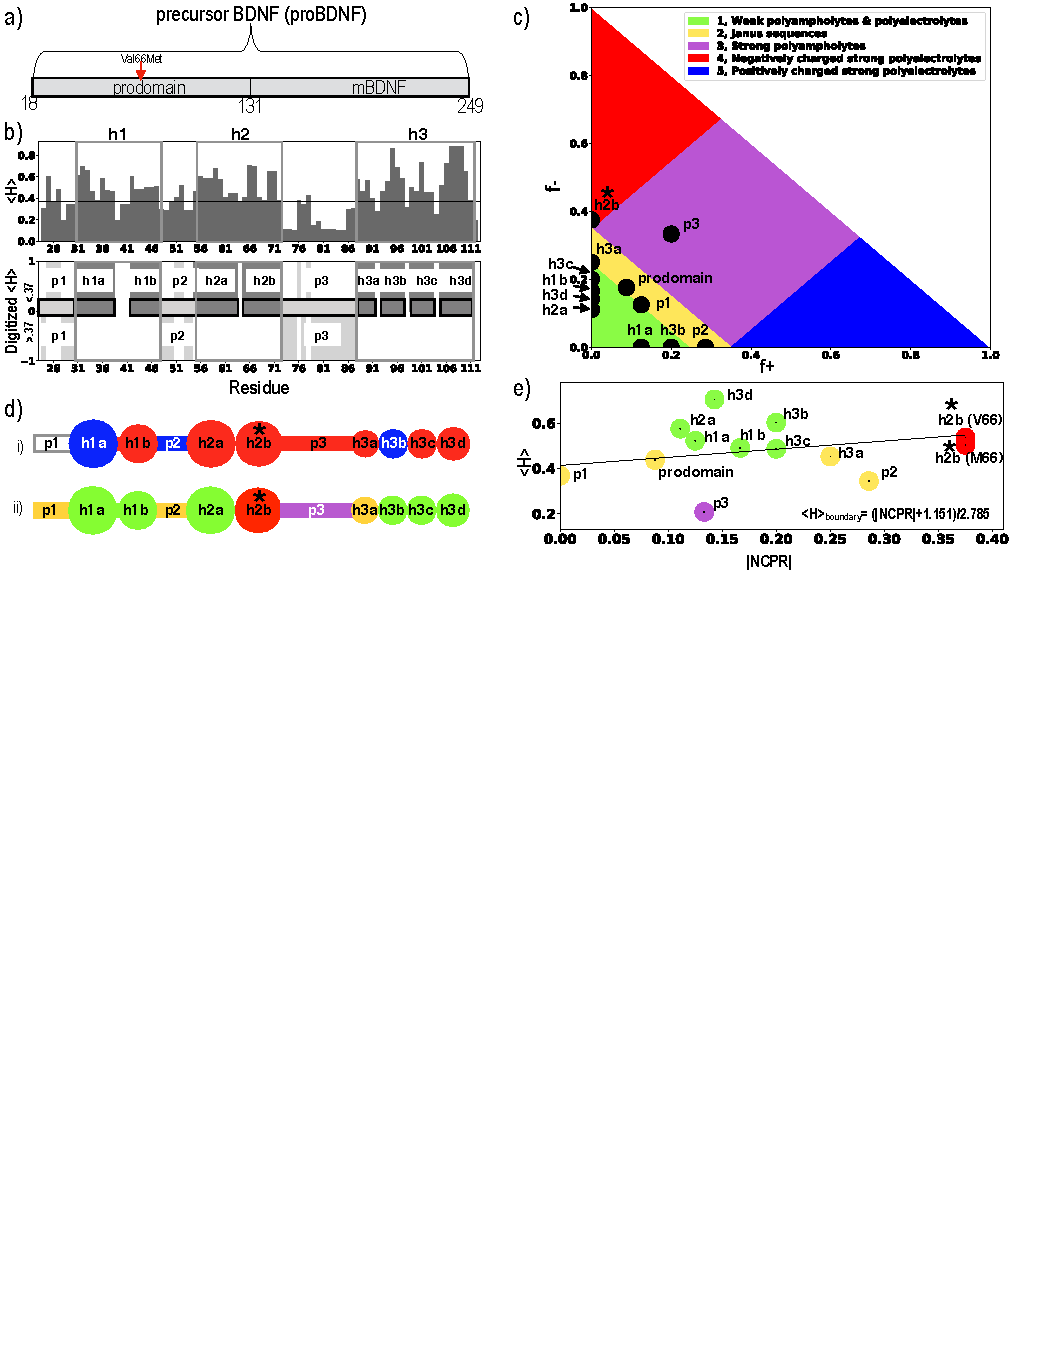
\includegraphics[scale=0.5,width=\textwidth,trim={0 0cm 0 0cm},clip]{../figures/fig1.pdf}
\caption{{\bf Prodomain and it's domain decomposition.} 
a) proBDNF consists of two domains: the prodomain and mature BDNF (mBDNF). b) Diagram of states reported by Ref.~\cite {Das2015,Das2013a}, based on fraction of positively and negatively-charged residues.  As indicated with star, the neutral and protonated BDNF prodomain lies in the Janus region.
c) Mean hydrophobicity for the V66 prodomain based on a sliding window of 3 residues (top) and hydrophobicity based domain identification of prodomain sequence (bottom) further described in methods. Eight hydrophobic domains (darkgrey) are identified along with 3 domain of low hydrophobicity (dimgrey). d) The cartoon representation of the prodoamin where i) domains colored according to net charge; negative charge (red), positive charge (blue) and neutral (white) ii) domains are colored according to the region found in diagram of states for neutral (top) and protonated prodomain (bottom). The domain h2b contains the mutation and is marked with star. Parts b) is generated with CIDER. ~\cite {Holehouse2017}}
\label{fig1} 
\end{figure}
%/todo increase the label spacing and switch the order for part c).
Difficulties in obtaining unambiguous disease associations at the proBDNF Val66Met mutation using GWAS are paralleled by challenges in characterizing its effects on the properties of the BDNF prodomain using structural techniques.  A crystal structure of a homologous neurotrophic factor in complex with a shared receptor, revealed a well-defined volume corresponding to the prodomain, but which lacked resolvable density.\cite{Feng2010a} 

It was subsequently revealed that the cleaved prodomains ($\sim90$ residues) are found in monomeric states {\it in vivo}, and the M66 (but not V66) form binds to SorCS2 (sortilin-related VPS10p domain containing receptor 2), leading to axonal growth cone retraction.\cite{Anastasia2013} NMR measurements on the prodomain confirmed significant intrinsic disorder for both forms, with differential secondary structure preference around residue 66. ~\cite {Anastasia2013}.  It was not possible to gain any insight into the BDNF prodomain tertiary ``structure'', with uncertainty in interpretation of NMR signal obscuring whether secondary structure is affected far from the mutation, but additional NMR experiments implicated residue 66 in binding of M66 prodomain 
 to SorCS2.~\cite {Anastasia2013}
 
The Val66Met is present in a region with high density of negative charged residues (D61,E64,E68,E69) (Fig~\ref{fig1}c). In this scenario, residue H65 can exist in protonated or neutral charge state in vivo due to it's low pKa. In order to capture the effects of histidine protonation states on Val66Met, we study the Val66 and M66 prodomain in presence of both neutral H65 and protonated H65. For the ease of understanding our observations, the prodomain sequence is divided into hydrophobic domains (Fig~\ref{fig1}c).

In this work, we report on unbiased fully-atomistic replica-exchange MD simulations of the 90 residue BDNF prodomain in explicit solvent, for V66,   V66\textsuperscript{65+}, M66 and  M66\textsuperscript{65+} forms.  This sequence falls at the boundary of the Janus and globular domains in the diagram proposed by Das and Pappu. \cite{Das2015,Das2013a} 

\section{Results and discussion}

%%%%%%%%%%%%%%%%%%%%%%%%%%
%1. Definition of Hydrophobic Domains, including some sequence analysis (kappa, f- f+ of individual domains)  (Figure 1)
%2. Comparison of experimental observables and their computational analogues (Figure 2)
%3. Computational Microscopy (expanded data for computational analogues to experimental results)  : Figure 3 and 4
%4. Discussion of Interdomain interactions (prototertiary structure):
%5. Discussion of Intradomain interactions (including length of secondary structures):
%6. Coupling between inter and intradomain interactions

\subsection{Prodomain Sequence Decomposition} 

%This subsection should at minimum answer the following questions : 

%-What was the motivation for dividing into domains (i.e. for coarse-graining the sequence)?
%-How do the different domains correspond to the Pappu phase diagram, and which type of domain does the mutation fall in? 
%-How is the SNP domain unique among the proBDNF domains? How is it that we can have a hydrophobic strong polyelectrolyte sequence? 
%-How are the Pappu domains arranged? (i.e. answer: with strong polyelectrolyte at center and globular domains on ends) 
% -What does coarse-graining the sequence reveal about the proBDNF sequence that isn't apparent from just looking at every residue individually? 


\begin{table}[ht]
\caption{Hydrophobic and linker domains identified in Pro region of BDNF\textsuperscript{\emph{a}}.}
\begin{center}
\begin{tabular}{|c|c|c|c|c|c|c|c|c|c|c|}
\hline
Domain &  N & NCPR  & $<$H$>$  & FCR  & f- & f+ & $\kappa$  & Sequence & R & P\\
\hline\hline
p-1 & 8 & 0.00 & 0.37 & 0.25 & 0.13 & 0.13 & 0.8 &  EANIRGQG & 2 & 0.00\\
\hline
h1a & 8 & 0.13 & 0.52 & 0.13 & 0.00 & 0.13 & 1.0 &  GLAYPGVR & 1 & 0.12\\
\hline
h1b & 6 & -0.17 & 0.49 & 0.17 & 0.17 & 0.00 & 0.1 &  TLESVN & 1 & 0.00\\
\hline
p1-2 & 7 & 0.29 & 0.33 & 0.29 & 0.00 & 0.29 & 1.0 &  PKAGSR & 2 & 0.16\\
\hline
h2a & 9 & -0.11 & 0.58 & 0.11 & 0.11 & 0.00 & 0.7 & GLTSLADTF & 1 & 0.00\\
\hline
h2b(V66) & 8 & -0.38 & 0.54& 0.38 & 0.38 & 0.00 & 0.3 &  HVIEELLD & 4 & 0.00\\
\hline
h2b(M66) & 8 & -0.38 & 0.50 & 0.38 & 0.38 & 0.00 & 0.3 &  HMIEELLD & 4 & 0.00\\
\hline
h2b\textsuperscript{65+}(V66)	&8	& -0.25&	0.54&	0.50&	0.38	&0.13	&0.6	&H\textsuperscript{+}VIEELLD	&3 & 0.00\\
\hline
h2b\textsuperscript{65+}(M66)	&8	& -0.25&	0.50 &	0.50&	0.38	&0.13	&0.6	&H\textsuperscript{+}MIEELLD	&3 & 0.00\\
\hline
p3 & 15 & -0.13 & 0.21 & 0.53 & 0.33 & 0.20 & 0.1 & \makecell{EDQKVRPI \\ NEENNKDA} & 3 & 0.06\\
\hline
h3a & 4 & -0.25 & 0.45 & 0.25 & 0.25 & 0.00 & N/A &  DLYT & 2 & 0.00\\
\hline
h3b & 5 & 0.20 & 0.60 & 0.20 & 0.00 & 0.20 & N/A &  RVMLS & 1 & 0.00\\
\hline
h3c & 5 & -0.20 & 0.49 & 0.20 & 0.20 & 0.00 &N/A &  QVPLE & 1 & 0.20\\
\hline
h3d & 7 & -0.14 & 0.70 & 0.14 & 0.14 & 0.00 & 1.0 &  PLLFLLE & 1& 0.14\\
\hline\hline\hline
V66 seq  & 91 & -0.09 & 0.44 & 0.26 & 0.2 & 0.09 & 0.2 & & 2 &0.07 \\
\hline
M66 seq & 91 & -0.09 & 0.44 & 0.26 & 0.2 & 0.09 & 0.2 & & 2 &0.07 \\
\hline
V66\textsuperscript{65+} seq & 91 & -0.08 & 0.44 & 0.28 & 0.18 & 0.10 & 0.2 & & 2 & 0.07\\
\hline
M66\textsuperscript{65+} seq & 91 & -0.08 & 0.44 & 0.28 & 0.18 & 0.10 & 0.2 & & 2 &0.07\\
\hline
\end{tabular}
\end{center}

\textsuperscript{\emph{a}}Number of residues (N), Net charge per residue (NCPR), Mean hydrophobicity  $<$H$>$, Fraction of charged residues (FCR), fraction of positive (f+) and negative charge residues (f-), $\kappa$ and region(R) in phase diagram as defined by Das et al ~\cite {Das2013a}, fraction of Proline residues (P). $\kappa$ was calculated using CIDER ~\cite {Holehouse2017}.


\label{default}

\end{table}
The BDNF prodomain is 91 residues long and residue-level analysis for the entire protein is challenging to interpret. To simplify analysis, the prodomain sequence was divided into subdomains based on sequence hydrophobicity. Eight hydrophobic domains (h) and 3 linkers with lower hydrophobicity (p) and higher disorder were identified (Fig~\ref{fig1}c). The properties of each domain are summarized (Table~\ref{default}).  

We characterized each domain on the phase diagram and calculated it's $\kappa$ as proposed by Pappu et al. ~\cite {Mao2010a,Das2013a}.  $\kappa$ measures charge segregation in a linear sequence; low $\kappa$ and high $\kappa$ is realized for well mixed sequences leading to random coil conformations and sequences with segregation of oppositely charged residues leading to hairpin like conformations, respectively. Two unique hydrophobic domains with high NCPR ($\geq$ 0.25) are identified: h2b/h2b\textsuperscript{65+} and h3a. 

The domain h2b has several unique properties: i) it contains the Val66Met mutation ii) is located at the sequence midpoint iii) its the only strong polyelectrolyte domain and has the highest NCPR among all the domains. It contains a mix of acidic and hydrophobic residues. Strong polyelectrolytes are predicted to behave as swollen coils~\cite {Das2013a}, thus the hydrophobic residues in this solvated expanded coil domain would be more accessible to the solvent than other hydrophobic residues in compact globule forming domains, if present as an isolated peptide. The Val66Met mutation slightly reduces the hydrophobicity of domain h2b (Table~\ref{default}). Protonation at residue His65 moves the entire h2b domain from a strong polyelectrolyte region with low $\kappa$ to a strong polyampholyte region with high $\kappa$.

The domain h3a is a unique hydrophobic Janus domain with high NCPR. Janus sequences have intermediate compositional biases and their conformations are context dependent ~\cite{Das2015b}. The SNP domain h2b and the Janus domain h3a are separated with the long (15 residue) strong polyampholyte linker p3 which has well mixed charge ($\kappa$ = 0.1). All remaining hydrophobic domains are classified as weak polyampholyte and are predicted to have compact globule conformations to shield hydrophobic residues if present as an isolated peptide ~\cite {Das2015b}. The domains h1a and h3b are positively charged and all the remaining hydrophobic domains are negatively charged (Fig~\ref{fig1}c).

The BDNF prodomain by itself is a boundary region polyampholyte with very low negative NCPR (Table~\ref{default}). However, by coarse-graining the BDNF sequence, we were able to identify it as an arrangement of eight hydrophobic domains interconnected by two less hydrophobic disorder promoting domains.
%Forty percent of IDPs reported in DISPROT are found to have compositions that place them in the boundary between globules and strong polyampholytes ~\cite {Das2015b}. 



%%%%%%%%%%%%%%%%%%%%%%%%%%%%%%
\subsection{Comparison of experimental observables and their computational analogues}

Chemical shifts for BDNF prodomain indicates very low propensity of residual secondary structure. In order to get accurate structural characterization of prodomain with MD,  we ran T-REMD simulations of 30 residue fragment of V66 prodomain with several commonly used forcefield and water model combinations. Amber99sb*-ildn-q ~\cite{Lindorff-Larsen2010a, Hornak2006a} with Tip4p-D ~\cite {Piana2015} yielded the best agreement with experimental data obtained by NMR ~\cite{Anastasia2013} (FigS1) and was used for the full prodomain simulations. This is consistent with the force field comparison study by Robustelli et al which observed that for IDP's with little or no secondary structure,  Amber99sb*-ildn-q with Tip4p-D gives good agreement with experimental NMR measurements ~\cite {Robustelli2018}.
\begin{figure}[!ht]
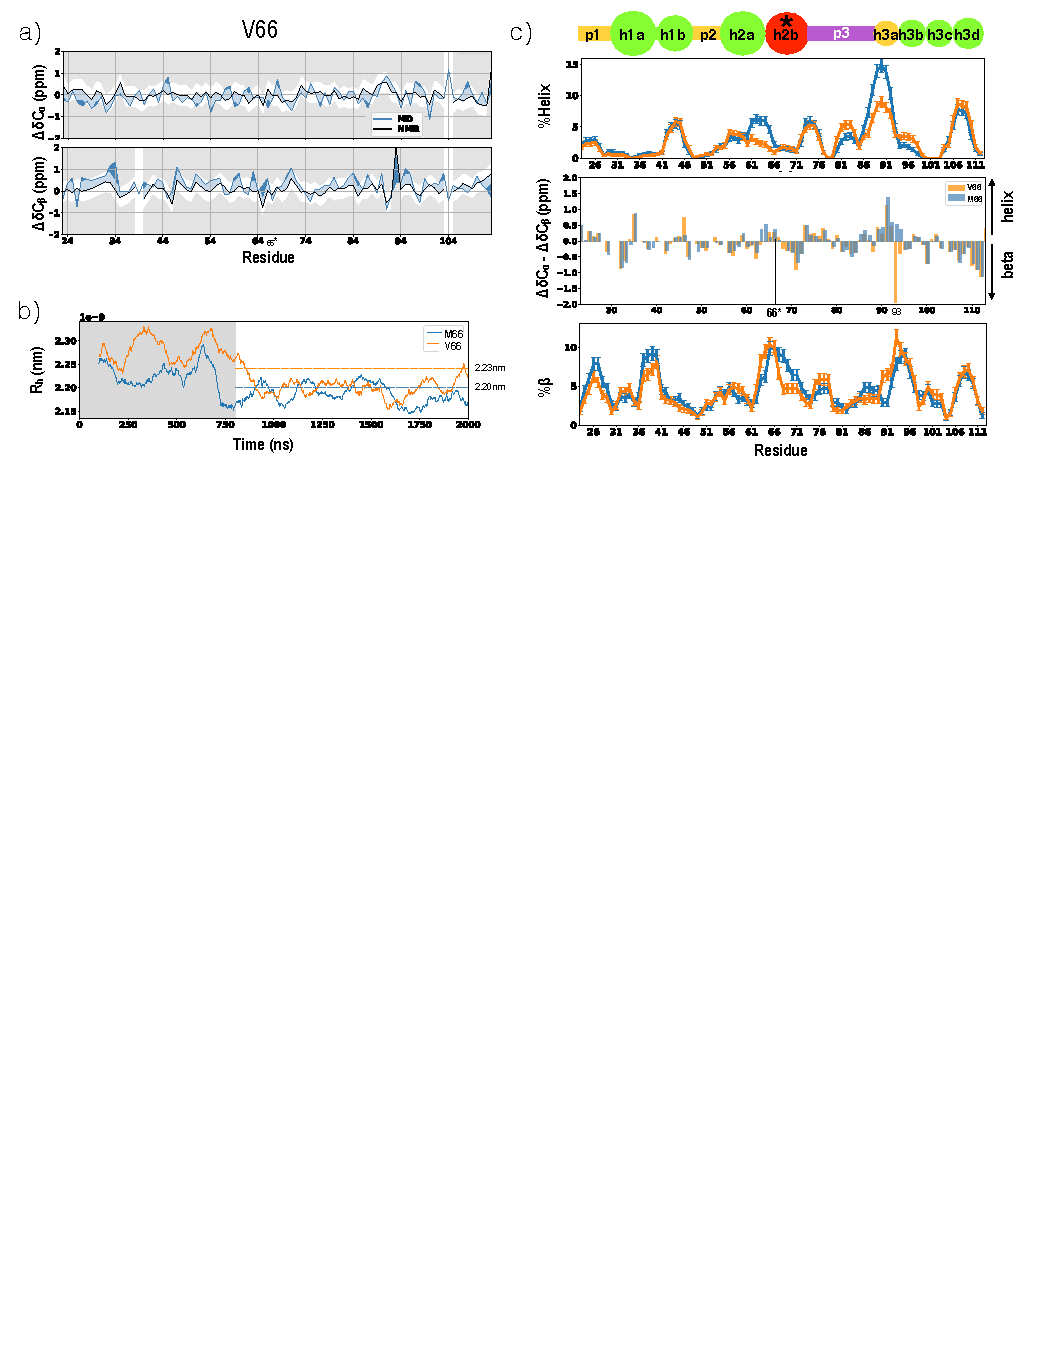
\includegraphics[scale=0.5,width=\textwidth,trim={0 0cm 0 0cm},clip]{../figures/fig2.pdf}
\caption{{\bf Comparison of MD and NMR observables.} a) Comparison of chemical shifts from MD ensembles (blue lines, at 300K) and NMR chemical shifts (black lines, at 280K) from Anastasia et al ~\cite{Anastasia2013}. b) Hydrodynamic radius (R\textsubscript{h}) at 100 ns moving  window for V66 and M66 sequence vs the simulation time. The R\textsubscript{h} for both the sequences converge after 800ns of simulation time. The NMR diffusion experiment values from Anastasia et al  ~\cite{Anastasia2013} are represented with dashed lines. c) Helix (top) or $\beta$ (bottom) propensity at each simulated residue defined as the probability of a given residue being part of a sequence of four or more consecutive residues whose dihedral angles place them in the helical region or beta region of the Ramachandran map (further described in methods). C\textsubscript{$\alpha$}-C\textsubscript{$\beta$} secondary chemical shifts for each sequence from Anastasia et al ~\cite{Anastasia2013} (middle). Positive differences indicate helical structure and negative differences indicate $\beta$ structure.}
\label{fig2} 
\end{figure}

In order to assess the validity of MD-generated ensembles, we compared the MD ensembles with experimental data obtained by NMR spectroscopy and NMR diffusion measurements (Fig~\ref{fig2}a,FigS2,FigS3a) . Fig~\ref{fig2}a shows the C\textsubscript{$\alpha$} chemical shifts calculated from the simulations using SPARTA+ ~\cite{Shen2010} and compares them with the NMR chemical shifts. We obtain good agreement with NMR chemical shifts: the discrepancy at each residue is \textless 0.7 ppm, which is less than the individual SPARTA+ prediction uncertainties of $\sim$ 1 ppm ~\cite{Shen2010}.

%Although there are some localized discrepancies for certain residue types (Y34,L59,M95,Y113), the discrepancy is conserved across all four simulations (FigS2). Thus, these specific discrepancies are probably reflecting residual force-field inaccuracies, including the cation-pi interactions that are poorly captured by non-polarizable force felid.
%this can be added only if I am comparing Cb chemical shifts
%todo Reference ?

The simulated hydrodynamic radii (R\textsubscript{h}) calculated using Hydropro ~\cite {Ortega2011} of V66 (2.23 $\pm{.02}$ nm) and M66 (2.20 $\pm{.02}$ nm) sequence are in excellent agreement with the experimental values from NMR diffusion measurements by Anastasia et. al ~\cite{Anastasia2013} (2.24 $\pm{0.1}$ nm and 2.20 $\pm{0.1}$ nm respectively) (Fig~\ref{fig2}b). The R\textsubscript{h} for protonated His65 (FigS3b) are also in excellent agreement with the experimental values (V66\textsuperscript{65+}:2.24 $\pm{.02}$ nm, M66\textsuperscript{65+}:2.21 $\pm{.02}$ nm). This approach has been used earlier to validate simulations of disordered proteins ~\cite {Rauscher2015, Meng2018} and our results support the use for Tip4p-D for such simulations ~\cite {Piana2015, Robustelli2018} .

Anastasia et al ~\cite{Anastasia2013} observed an increase in helical tendency for the M66 sequence within domain h2 and h3ab and an increase in $\beta$ tendency within domain h3b in the V66 sequence (Fig~\ref{fig2}c). 
To investigate the effect of the mutation on residual secondary structure for the simulated prodomain, we compared the helix tendency at every residue for V66 and M66 simulations (Fig~\ref{fig2}c). 

Consistent with NMR experiments, the M66 sequence demonstrates an increased tendency of forming helices within domain h2 and h3ab relative to the same domains in the V66 sequence (Fig~\ref{fig2}d). We also find that the residue R93 in domain h3b of V66 sequence has a higher tendency to form $\beta$-sheets than in the M66 sequence, in agreement with NMR experiments (Fig~\ref{fig2}c). We get consistent observations with NMR data ~\cite{Anastasia2013} when V66\textsuperscript{65+} and M66\textsuperscript{65+} simulations are compared (FigS3c).
 
%todo for comparing MD and NMR secondary structure I need to do d2D calcualtions
%For comparison, you could also calculate the mean of non-protonated and protonated form.

%%%%%%%%%%%%%%%%%%%%

\subsection{Interdomain interactions (prototertiary structure)}

%--------- domain level
%change the cutoff in contact maps
%--Purely based on the domain properties (not individual residue stuff yet), what interdomain interaction preferences would we expect (if any)?
%--What do we actually observe (in the WT, ancestral version)
%--Does it agree with our expectation?
%--How does the V66M hydrophobic mutation change these preferential interactions?  (Not "why" yet, just how)
%--V66M doesn't change any of the domain properties (does it?) - is there still a way for us to interpret  preferential interactions purely on the domain level? (i.e. h3a  is Janus sequence which is highly sensitive to small changes in interactions)
%--How does  65+  change  interdomain interactions, and is it consistent with what we'd expect based on how it affects properties of domain 2b?
%--Are changes in interdomain interactions consistent with changes in radius of gyration?
%a metric for the strongest contact formed in each domain

\begin{figure}[!ht]
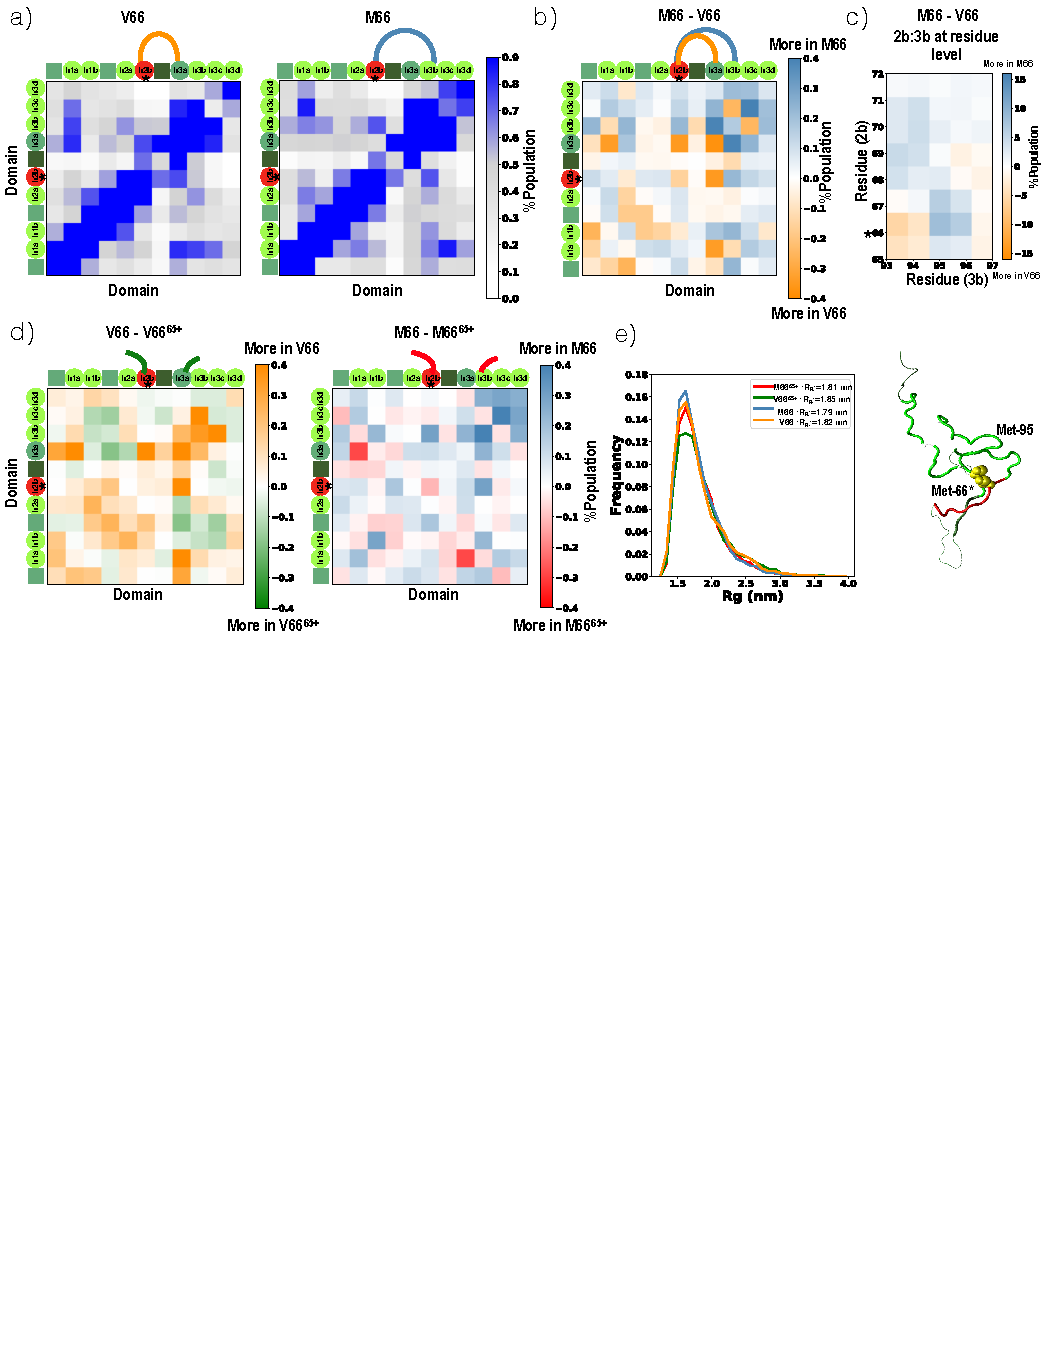
\includegraphics[scale=0.5,width=\textwidth,trim={0 0cm 0 0cm},clip]{../figures/fig-3.pdf}
\caption{{\bf Effect of Val66Met on inter-domain contacts.} a) Inter-domain contact probability for V66 (left) and M66 (right). The maps are annotated with cartoon representation of the prodomain; circles and squares represent hydrophobic domains and linker regions respectively and are colored as in Fig1. Two domains are in contact if the distance between any inter-domain pair of C\textsubscript{$\alpha$} atoms is within 8\AA. The contact probability for any domain pair is also normalized with the product of length of each domain. The most frequent long-range contact formed by the SNP domain is represented with an orange (V66) or blue (M66) edge connecting the two domains.  b) Difference between the contact probabilities shown in a); interactions more frequently found in M66 or V66 are in blue and orange respectively. c) Contact probability at each residue shown in b) within domains h2b and h3b (top). Representative conformation of M66 sequence showing Met66-Met95 contact, colored as in Fig1 with Methionine in yellow. Thick lines represents hydrophobic domains whereas thin line represents linker regions (bottom). d) Difference between the contact probabilities of neutral H65 and protonated H65 for V66 (left) and M66 (right) sequence respectively. e) R\textsubscript{g}) distributions across all four simulations.
 }
\label{fig4m}
\end{figure}
To identify favorable long-range interactions we calculated the normalized probability of inter-domain C\textsubscript{$\alpha$} interactions (Fig~\ref{fig4m}a, FigS5a) as described in the Methods. We find that hydrophobic domains have a higher probability of forming long-range contacts, even for domains separated by sequence. The inter-domain contacts for the least hydrophobic, strong polyampholyte p3 linker decay with the distance along the sequence as we would expect for a random coil. 

Two out of 8 hydrophobic domains in the prodomain are positively charged, and all the remaining domains are negatively charged. Consistently, most of the observed long-range contacts either include positively charged domains h1a or h3b  and/or negatively-charged, high NCPR domains, h2b and/or h3a (Fig~\ref{fig4m}a, FigS5a). Furthermore, the oppositely charged terminal domains have frequent contacts. Overall, we find that even for hydrophobic domains, electrostatic interactions do contribute to inter-domain contacts.


We find that frequent contacts are always formed between neighboring domains, except at h2b/h2b\textsuperscript{65+}-p3 and h3c-h3d. Three sequential same charged residues (Asp72,Glu73,Asp74) at the interface between h2b/h2b\textsuperscript{65+} and p3 and two sequential Proline residues (Pro104,Pro105) at the interface between h3b and h3d probably explains the less frequent contacts between these two neighboring domains (Table~\ref{default}). We would expect the strong hydrophobic polyelectrolyte h2b domain to form frequent contacts with all other domains, due its exposed hydrophobic residues and low $\kappa$ (Table~\ref{default}). Indeed, the SNP domain h2b forms strong long range contacts with positively charged domain h3b and/or the negatively charged h3a.

In order to understand the effect of Val66Met on inter-domain contacts, we compared the contact maps for each sequence (Fig~\ref{fig4m}b). Val66Met shifts the inter-domain h2b-h3a contact to h2b-h3b. 
To understand the origin of the more favorable interaction between the SNP domain and h3b, we zoom in on the residue level interactions between these two domains (Fig~\ref{fig4m}c). Both V66 and M66 sequence form their strongest interactions between hydrophobic residues, Val66-Val94 (9\%) and Met66-Met95 (10\%) respectively (FigS4). Interestingly, we find that Met95 forms frequent contact with Met66 and not Val66 (Met66-Met95 (10\%) vs Val66-Val95 (2\%)). This is consistent with the results of ab-initio calculations: Gomez-Tamayo et al has reported that Met-Met interactions are stronger than Met-Leu, Met-Phe or aromatic-aromatic interactions due to polarizability of sulphur ~\cite{Gomez-Tamayo2016}.

Apart from direct effects on contacts involving SNP, we also observe indirect effects on contacts not involving the SNP. h3a-h3b and h3a-h1a are observed frequently in M66 and V66 sequence respectively (Fig~\ref{fig4m}b). Even when H65 is protonated, Val66Met changes the maximum contact preference for the Janus domain h3a; gain of contacts at h3a-h3b, h3a-h1a and loss of h3a-h2a in M66\textsuperscript{65+} when compared with V66\textsuperscript{65+} (FigS5b). 

In order to understand the effect of protonation on the prodomain ensemble, we compared the inter-domain contact maps for each protonation state (Fig~\ref{fig4m}d). h2b\textsuperscript{65+} forms fewer contacts with the remaining domains for both V66 and M66 when compared with h2b. Infact, we observe more self-interactions of h2b\textsuperscript{65+}, as expected for a strong polyampholyte domain with high $\kappa$ when compared with strong polyelectrolyte domain with low $\kappa$ (Table~\ref{default}). 
Apart from direct effects on contacts involving h2b\textsuperscript{65+}, protonation causes loss and gain of h3a-h1a contacts in V66 and M66 sequences respectively. This sensitivity to both mutation and protonation of other domains is consistent with context dependence of the Janus sequence h3a.

There are slight differences in the radius of gyration (R\textsubscript{g}) distributions across all four simulations (Fig~\ref{fig4m}e): 1) The sequence with Met66 has slightly lower R\textsubscript{g} when compared with its Val66 form. For M66 sequence, the SNP domain h2b/h2b\textsuperscript{65+} forms frequent contacts with the rest of the domains when compared with the Val66 sequence(Fig~\ref{fig4m}b). This could explain the slightly more compact states of M66 and M66\textsuperscript{65+}  when compared with V66 and V66\textsuperscript{65+}. 2) The His65 protonated form is more expanded when compared with its respective non-protonated states. For both V66 and M66 sequence, protonation at 65 reduces inter-domain contacts at h2b (Fig~\ref{fig4m}d), which is consistent with the slight increase in R\textsubscript{g} upon protonation.


%%%%%%%%%%%%%%%%%%%%%%%%%%%%%%%%%%%%INTRADOMAIN%%%%%%%%%%%%%%%%%%%%%%%%%%%%%%
\subsection{Intradomain interactions and residual secondary structure}
%QUESTIONS: 
%In what way does the residual secondary structure in the vicinity of the mutation/protonation site change? 
%In what way does the length of secondary structure elements change? 
%What could explain these differences (without -yet- invoking interactions with other domains)?
%END QUESTIONS
%I think you should be pretty comfortable with this section, but you should to restrict them to h2b  and 3a, and consider them separately
We find frequent intra-domain contact probablity at every domain except at p3 linker and domain h3c (Fig~\ref{fig4m}a, FigS5a). Consistent with p3 linker being a strong polyampholyte with low $\kappa$, we find less self interaction in this domain (Table~\ref{default}). Domain h3c show less self-interaction due to it's highest fraction of Proline (20\%) and it's placement at the center of the domain (Table~\ref{default}).

The NMR chemical shifts indicate that mutation increases the helicity at both the SNP domain h2b and Janus domain h3a. In agreement with NMR, we find an increase in helical structure at both domains in the M66 sequence (Fig~\ref{fig1}c). Comparing the length of secondary structure formed at each residue (Fig~\ref{fig4}a,FigS8b) reveals an even stronger effect of the mutation: in both protonated and neutral His65 states, Val66Met consistently increases the frequency of long helix formed within domain h2. 
%Strikingly, we find that only Met66 and not V66 forms long helical structures of 4 or more residues at the SNP domain (2a,2b) (Fig~\ref{fig4}a). We observe likewise for M\textsuperscript{65+}. 

\begin{figure}[!ht]
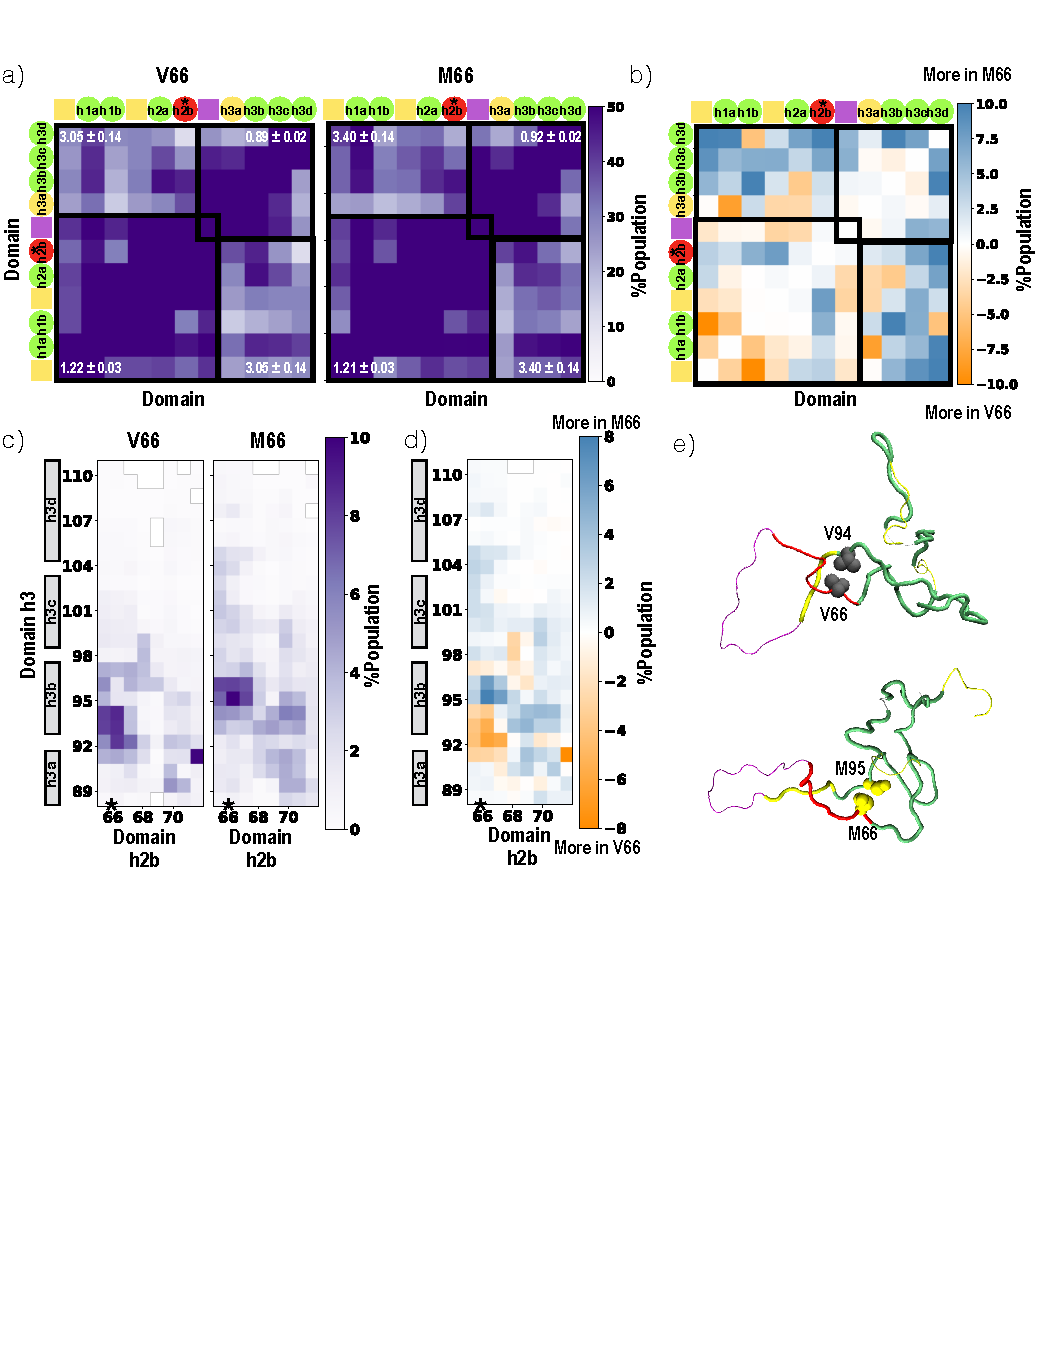
\includegraphics[scale=0.5,width=\textwidth,trim={0 0cm 0 0cm},clip]{../figures/fig4.pdf}

\caption{a) Difference in helix length probability at each residue in the prodomain. b) Intra-domain contact probability for V66 (left) and M66 (right). Each residue in domain 2 is annotated with a circle representation and the most preferred contact is represented with an edge. c) Difference between the contact probabilities shown in b); interactions more frequently found in M66 or V66 are in blue and orange respectively. }

\label{fig4} 
\end{figure}

Reduced entropic cost of helix formation in M66 when compared with V66 possibly contributes to the increased helix formation in the h2 domain. Creamer et. al. ranked the entropic cost of helix formation for apolar side chains using simulations of a (Ala)\textsubscript{8} sequence with the guest amino acid at the center, and reported higher entropic cost of helix formation for Valine when compared with Methionine\cite{Creamer1992}. In general, C\textsuperscript{$\beta$}-branched amino acids, such as Valine, have more restricted side-chain rotamers in helical conformation when compared with non-C\textsuperscript{$\beta$}-branched amino acids.

The helical structure in M66 is also stabilized by local sequence.  \ruchi{ We considered the intra-domain contact map of domain h2 and find that for both M66 and M66\textsuperscript{65+}, Met66(i) is frequently contacting Phe63(i-3) when compared with any other intra-domain contact at residue 66: M66-F63 is 50\% stronger when compared with M66-E69 (Fig~\ref{fig4}b,FigS8b). } In the V66 sequence, it is far more likely that the Ile67(i+1)-Leu70(i+4) contact is formed (Fig~\ref{fig4}c).
A previous study from Faure et al ~\cite {Faure2008} analyzed the frequency of two amino-acids contact within 1230 protein chains from the Protein DataBank (PDB) and found that Met has also a strong affinity for Phe and other Methionines. In fact, we find that the largest change in intra-domain contacts from V66 to M66 is the gain of contact at M66-F63 (20\% stronger in M66 when compared with V66) followed by loss of contact at Ile67(i+1)-Leu70(i+4) (Fig~\ref{fig4}b). 
% (also add the reference for sulphur stabilizing helical conformation. 

When the M66 sequence is protonated at His65, the helix propensity shifts from helix at residues 59-66 to even longer helix at residues 59 - 69 (Fig S8a). When protonated, both V66 and M66 sequences gain contacts with His65,Met/Val66 and Ile67 (FigS8b). These increases in intra-domain contact frequency at h2b\textsuperscript{65+} are consistent with expectations, since protonation at H65 reduces the net charge and increases $\kappa$ of the otherwise negatively charged polyeletrolyte domain with low $\kappa$ (Table~\ref{default}). 


%Among all intra-domain contacts, all four simulations has stretch of strong contacts formed at i:i+3. Two hydrophobic residues commonly form strong contacts (\textgreater 60\%) among all residue pairs. A60:F63 forms strong contact for all four simulations. 
 
%Among others 
%\subsubsection{Janus domain}
%QUESTIONS:
%In what way does the residual secondary structure or length of secondary structure elements change for each mutation and protonation state? (i.e. what should the reader be noticing)
%It was placed in the Janus sequence region based on f+ and f-, so are the changes in secondary structure associated with differences in interactions between charged residues? 
%END QUESTIONS
\clearpage

\subsection{Secondary structure (intra-domain) and tertiary structure (inter-domain) coupling} 

%%%%Questions
% 1) In V66, there is a much stronger contact between h2b  and h3a  than in any of the other systems.  Are there ways in which the h2b  or h3a  intradomain interactions are also different for V66 from any of the other systems? [Provide 1-3 ways] 
% 2) For each difference, does the difference/correlation extend to fluctuations within the V66 sequence? (for example, one way might be that h3a  is also much less likely to form helix in V66 than the other sequences. Considering just the V66 simulation, for frames when 2b-3a contact is formed, are h3a  helices shorter/less probable than frames when no 2b-3a contact is formed?) 

%%%ON HOLD for now%---------residue level
%--Do the specific residues participating in interactions change for V66M, *particularly* *between within h2b  and 3a*
%--(optional) Do the specific residues participating in interactions change for 65+, *particularly* *between within h2b  and 3a* (edited).
\begin{figure}[!ht]
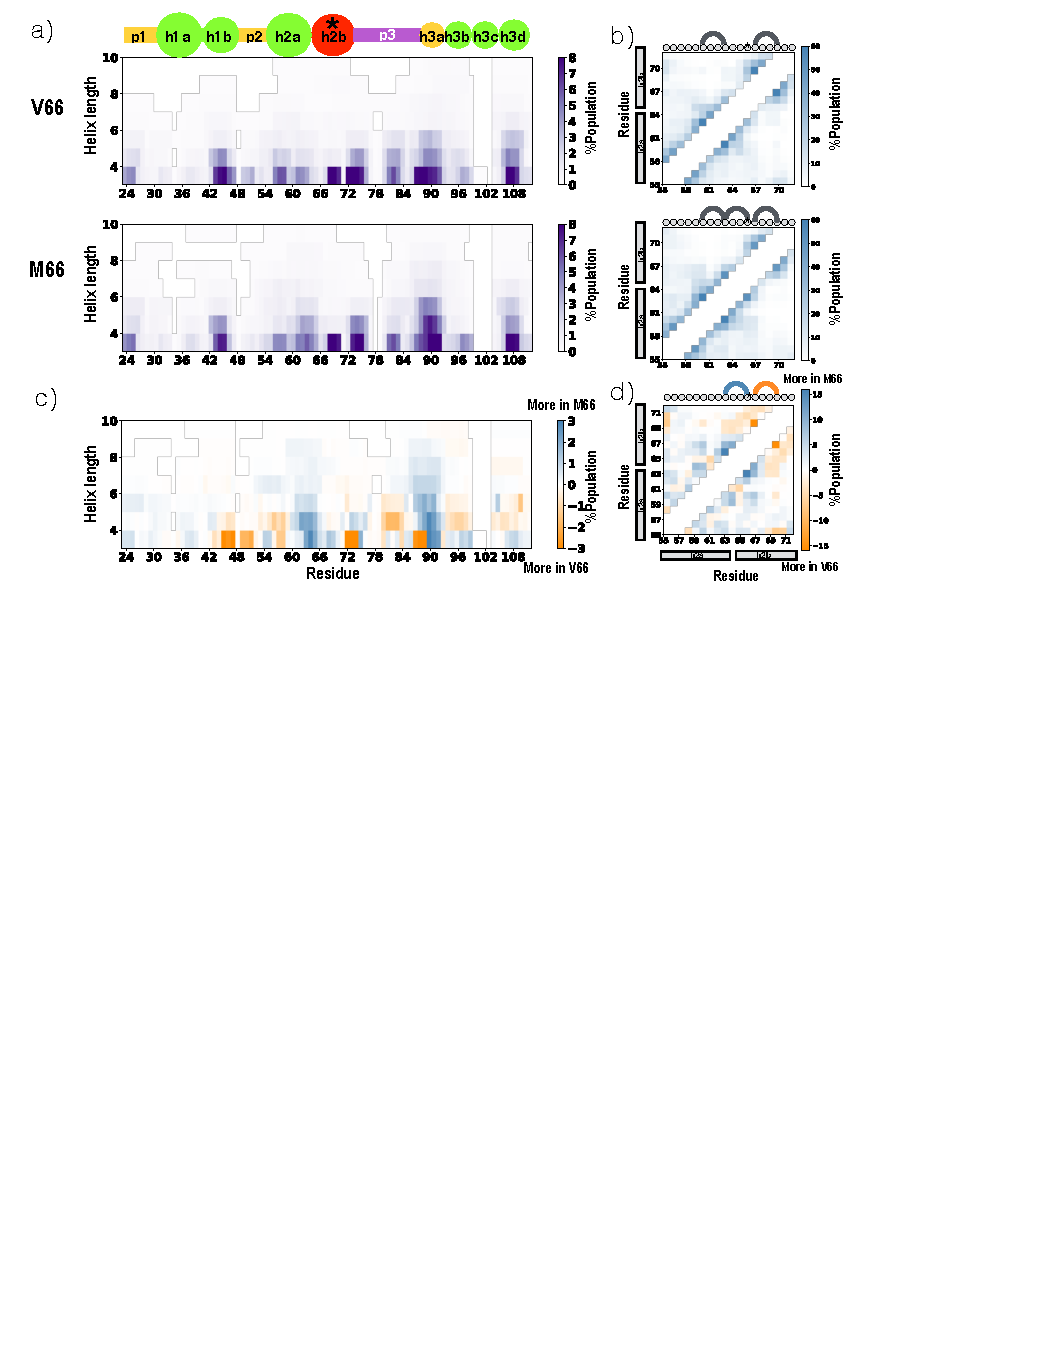
\includegraphics[scale=0.5,width=\textwidth,trim={0 0cm 0 0cm},clip]{../figures/fig5.pdf}
\caption{{\bf h2b-h3ab contact in prodomain and domain h2 secondary structure coupling.} Helix (a) and $\beta$ (b) propensities at each residue in V66(top) and M66(bottom). Frames were first clustered by whether the inter-domain h2b-h3a (left) or h2b-h3b (right) contact was formed (blue) or broken (orange), and then by whether the respective secondary structure was present in h2b (solid) or absent (dashed). 
 }
\label{fig5}
\end{figure}

Both our own MD results and previous results from NMR indicate the mutation causes local secondary structure change in domain h2 and non-local secondary structure changes in domain h3a and h3b (Fig~\ref{fig4}c). We hypothesized that since the Val66Met mutation affects the contact frequency of domain h2b with h3ab, the secondary structure change in h3ab could be due entirely to the change in inter-domain contacts. To test this, we divided the frames into 4 clusters, representing two independent collective variables with two possible values each: either the inter-domain contact is formed or broken, and either domain h2 does or does not have significant secondary structure.



First, we clustered frames by whether the SNP domain h2b is in contact with h3ab and then by whether helical structure was present in h2. Fig~\ref{fig5} compares the helix propensities at each residue for each cluster in V66 and M66 sequence. In V66 sequence, formation of h2b-h3a and/or h2b-h3b disrupts helicity at residue 66 and within Janus domain. We observe likewise for V66 protonated sequence (FigS11). In M66 sequence, we find that both the contacts h2b-h3a and h2b-h3b stabilizes helicity at residue 66. Additionally, when h2b-h3a is formed, the domain h3a helix has twice as much probability to be formed simultaneously with h2 helix when compared with the remaining 3 clusters Fig~\ref{fig5}. This suggests that the h2b-h3a inter-domain contact is necessary but not sufficient for increased helix formation in h3a. We observe likewise for M66 protonated sequence (FigS11b). 

Next, we looked at the 4 clusters made with $\beta$ structure at h2 as dependent variable for each contact (Fig~\ref{fig5}b). In V66 sequence, we find that both the contacts h2b-h3a and h2b-h3b stabilizes beta at either domains. Additionally,  when h2b-h3b is formed,  the domain h3b $\beta$ has much stronger correlation with domain h2 $\beta$ when compared with the remaining 3 clusters Fig~\ref{fig5}. This suggests that the h2b-h3b inter-domain contact is necessary but not sufficient for increased $\beta$ formation in h3b. In M66 sequence, we do not observe any such correlation.

\begin{figure}[!ht]
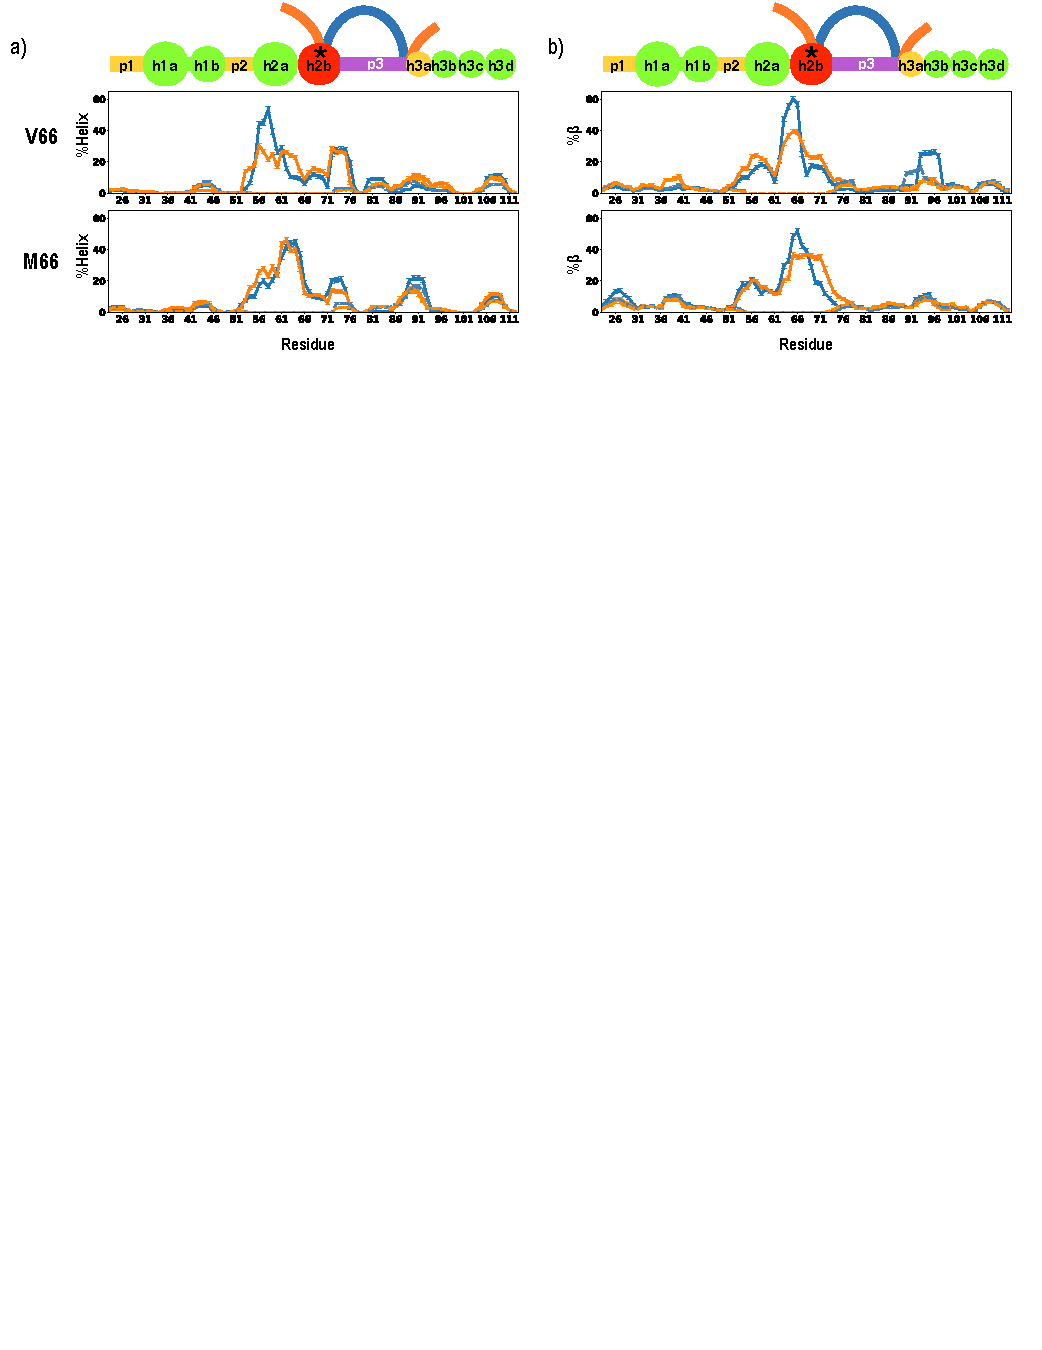
\includegraphics[scale=0.5,width=0.5\textwidth,trim={0 0cm 0 0cm},clip]{../figures/fig6.pdf}
\caption{{\bf Intra-domain and inter-domain contacts at residue level.} Difference between contact probability for M66 and V66 sequence at each residue in domain h2 when inter-domain contact is present between h2b-h3a (left) and h2b-h3b (right). The strongest contact difference is represented with an orange (V66) or blue (M66) edge connecting the two residues. b) Contact probability at each residue between domains h2 and h3ab when helix (b) or $\beta$ (c) within domain h2 is formed in V66 and M66 sequence respectively. Preferred hydrophobic interactions are annotated with black squares, backbone contacts with green squares and opposite charge contacts with red squares. The label of the plots are colored according to residue type: blue-basic, red-acidic, green-polar and Gly, grey-hydrophobic. i) and ii) are representative conformations from 2 different replicas for V66 (left) and M66(right) with chain colored as in Fig1 and preferred residue-level contacts in VDW representations, with residues colored with residue type.}
\label{fig6}
\end{figure}

To summarize, we find that the direct contact between the SNP domain and h3ab predicts $\beta$ and helicity locally in V66 and M66 sequence respectively. This was further confirmed by looking at the intra-domain contact probability within h2 when either contact is formed for V66 vs M66 sequence (Fig~\ref{fig6}a). M66 sequence forms helix supporting contacts at residue 66(i) whereas V66 doesn't form any strong intra-domain contact at 66 when h2b-h3ab is formed.
For non-local secondary structure change at h3ab, the h2b-h3ab inter-domain contact is necessary and but is not sufficient. Intra-domain contact at h2 influences intra-domain contact at h3ab when h2b-h3ab inter-domain contact is formed.

Few studies have reported helix-helix stabilization in IDP's. Feuerstein et al ~\cite {Feuerstein2012} reported partly stabilized helical structure by long-range tertiary in disordered fragment of the hepatitis C virus protein NS5A with PRE measurement from NMR. Conicella et al. ~\cite {AlexanderConicella2016} showed that TDP-43 undergoes liquid-liquid phase separation in part via helical contacts that are enhanced by self-interaction and can be disrupted by disease mutation. However, identifying the type of interaction at residue level has been difficult due to disorder.

To determine the type of residue contacts between h2 and h3ab stabilizing $\beta$ and helicity in V66 and M66 sequence, we plotted the inter-domain contact probability when respective secondary structure is formed at h2(Fig~\ref{fig6}a). In V66 the beta pairing at h2b-h3b is supported via combination of backbone hydrogen bonds at V66:S92, electrostatic and hydrophobic contacts at residues E64:R93, V66:V94 respectively (Fig~\ref{fig6}b). We do not find these beta sheet structures with h2b:h3a contact in V66 protonated states (Fig S10,S12). This is likely due to electrostatic repulsions between residue H65+ and R93.
In M66 the helix coupling of h2b-h3ab is supported via hydrophobic contacts at residues M66 and L70 (Fig~\ref{fig6}c). In protonated states, helix within h3ab is supported via hydrophobic contact with residue M66 as well (FigS11c).


\clearpage

%\textbf{In V66 when 2b:3b are in contact, there is formation of beta structures}\\
%Inter-domain contacts (residue level): V66:S92 is formed. This supports beta structure at residue 66.\\
%Intra-domain contacts: In V66, I67:L70 is present in domain 2b.\\
%In the above results we found that V66 intradomain interaction is unique; it has the weaker intradomain contact at 63:66 and stronger intradomain contact at 67:70.  V66 also has the weakest probability of helix formation at 66. In quantative terms, V66 has 50\% higher probability of contacts when 63:66 is absent and 67:70 is present simultaneously when compared with other three simulations (40\% vs 20\%).\\
%probability is directly proportional to sample size
%2b:3a forms strong contact in V66 when compared to any other simulations. 50\% of the contacts formed at 2b:3a is formed simultaneously with the absence of 63:66 and formation of 67:70. At domain 3a:3b, the contact 90:93 breaks when 2a:3b is formed in V66.\\
%We next examined the increased helix tendency at residue 93 from Val66Met substitution. We find structures forming helix at 93 are in contact with residue 66 in at-least 25\% of it's population in M66\textsuperscript{65+} (Fig~\ref{fig6}). The gain of this residue specific interaction in M66, probably increases helix formation at 93 when compared with V66. 


\section*{Summary and Conclusion}

We have carried out $\sim$ 0.5ms of fully-atomistic MD simulation of the 91 residue prodomain of brain-derived neurotrophic factor with protonated and neutral His65 state, both with and without the disease-associated Val66Met mutation. These long simulations successfully reproduced the experimentally observed chemical shift and R\textsubscript{h}. In respect to effect of the Val66Met mutation on residual secondary structure observed experimentally, the simulations were able to correctly reproduce the location of both local and non-local secondary changes due to the Val66Met mutation in the prodomain sequence. 

%We find that the highly disordered long prodomain, which by itself is a Janus sequence IDP can be meaningfully divided into domains based on sequence hydrophobicity alone.    

Due to highly dynamic nature of disordered proteins, identifying their tertiary contacts preference is very challenging. In this study, we showed that coarse-graining a highly disordered long prodomain into domains of 4 or more residues based on the hydrophobic residues distribution along the sequence can give us meaningful insights into it's "tertiary" contact network. 

We show that the intra-domain and inter-domain contact frequency at each domain is determined by it's mean hydrophobicity in addiction to NCPR, charge residue distribution as proposed by Das et al. and it's proline content.

Each identified hydrophobic domains lie in the folded protein region in the mean charge vs mean hydrophobicity plot except the linker domain p3. We identified two unique hydrophobic domains, the Val66Met mutation containing strong polyelectrolyte domain h2a and the Janus domain h3a connected via a unique highly disordered long linker region p3. These unique domains have biological significance as well: The sequence h2-p3-h3abc is essential for intracellular trafficking of proBDNF ~\cite {Chen2005}. 

The functional importance of flexible linker regions in ordered has been intensively analyzed. Flexible linkers allow the connecting domains to freely twist and rotate to recruit their binding partners in ordered proteins. The presence of linker region at the separation of SNP domain and h3ab is probably essential in this protein design.

In alignment with the sequence characteristics of Janus sequences, we find that Janus domains has the unique ability to forms both helix or $\beta$ structures with high propensity. We observe that Janus domain secondary structure and inter-domain contacts is sensitive to SNP domain secondary structure and mutation/protonation within SNP domain respectively. 

%We find that Val66Met mutation lies in a unique strong polyelectrolyte and hydrophobic domain of the prodomain. Thus, it is likely that the hydrophobic residues in the SNP domain is more accessible to solvent/rest of the domains when compared with accessibility of hydrophobic residues in any other domains. 

At residue level tertiary contact preference, we observe that Met-Met interactions drives tertiary contact changes in the prodomain due to Val66Met. Met-Met interactions have been shown to stabilize tertiary contacts in folded proteins and membrane proteins, but their role has not been investigated in disordered proteins. When the adjacent histidine is protonated, the frequency of tertiary contacts are reduced, including Met-Met interactions. This is likely due to less exposed hydrophobic residues in now strong polyampholyte SNP domain when compared with polyelectrolyte SNP. This suggests that Met-Met interactions could play a role in IDP tertiary contacts if present in a polyelectrolyte/expanded coil conformation region.

Interestingly, we find that for non-local secondary structure change, the inter-domain contact between local and non-local domain is necessary and but is not sufficient. Intra-domain contact at local domain influences intra-domain contact at non-local domain when inter-domain contact is formed between the two domains. Staller et al ~\cite {Staller2018} have earlier reported that in disordered acidic activation domain (Gcn4), the acidic residues keep key hydrophobic residues exposed to solvent and binding partners. In M66, mutation-Janus stabilizes helix structures in either domain mediated via hydrophobic interactions, whereas in V66, mutation-Janus stabilizes $\beta$ structures within Janus domain mediated via combination of backbone hydrogen bonding, hydrophobic and electrostatics.

%When protonated, both V66 and M66 sequence, loses most $\beta$ propensity within the SNP. The helix coupling within mutation and Janus domain is in-sensitive to protonation in M66 sequence. However, protonated Val66 sequence, loses most $\beta$ coupling at h2b:h3b, probably due to loss of the salt-bridge at E64:R93. V66\textsuperscript{65+}, the negatively charged Janus domain h3a forms $\beta$ structures with positively Janus 1-2 linker region. This is not surprising, since 1-2 linker and h3a are oppositely charged domains with high NCPR (Fig S12). 

We were able to get insights into the mechanism via which hydrophobic mutations can have effects on proteins secondary structure, non-local secondary structure and tertiary contacts. We compare the effects of a hydrophobic mutation and adjacent histidine protonation. i) Mutation changes tertiary contact preference via Met-Met interactions. Whereas, protonation weakens inter-domain contact ii) Mutation changes intra-domain contact preference due to local sequence effects and residue entropic cost of helix formation. Protonation increases intra-domain contact frequency due to reduced electrostatic repulsions in the otherwise negatively charged SNP domain.

%Instead of differences, talk about the similarity between hydrophobic and charged residue mutations in general.

Anastasia et al~\cite{Anastasia2013} observed differential kinetics for interactions between the BDNF prodomain and SorCS2; M66 binds more preferably at SNP domain (H65 to L71) with SorCS2, whereas V66 binds weakly overall but more strongly with domain h3a and h3b  (residues Y90 to V94). 
The stronger binding at residue M66 could be attributed to either a) ability of M66 to form alpha-helix at residue 66 when compared with V66 or b) stronger Met-Met contact at residue M66 with the SorCS2 Met residues, or a combination of both a) and b). 

In our simulations, we observe that helicity within the SNP domain is coupled with contact formation between the SNP domain and Janus domain hydrophobic residues. The SorCS2 sequence also has a Janus domain patch on it's surface. Thus, M66 forms could form simultaneous helix and contact formation within the SNP domain and Janus domain on SorCS2 surface. In V66, instead of the SNP, the Janus domain may interacts strongly with SorCS2 surface.

Protonation increases self interaction but reduces inter-domain contacts, thus, very slightly low pH can mediate the interaction between the SNP domain and SorCS2 surface. 

\section*{Materials and Methods}

\subsection*{System setup} To account for differences in starting coil conformation, we included six unique structures to represent residues 23-113 of BDNF prodomain.  All structures were built using I-Tasser ~\cite{Yang2014,Roy2010,Bioinformatics}, Robetta and Modeller ~\cite{Sali1993a}, and all were simulated in a water box at 600K for 50 ns at a constant volume. From the six resulting trajectories, 64 structures with correct proline isomers were selected (based on at least 2ps time interval); in total, our study included 64 unique prodomain structures. All structures were cooled to 300K for 1ns, while prolines were restrained in trans-conformation. Each V66-Hip65 replica was placed in a dodecahedron water box with 30,500 TIP4P-D ~\cite {Jorgensen1983} water molecules and a 0.15M salt concentration (NaCl) for a total system size of approximately 124,000 atoms. The same volume for each replica was ensured by fixing the simulation box of each replica to the average box size (11 nm).

\subsubsection*{Molecular Dynamics Simulation} For the simulations we use the amber99SB*-ILDN-q force field\cite{Lindorff-Larsen} and the GROMACS 5.1.2 simulation package,\cite{Berendsen1995,Abraham2015}, with a time step of 2 fs. 64 replicas are used with temperatures ranging from 300-385K, with exponential spacing. System was simulated using T-REMD \cite{Sugita1999a} with an exchange frequency of 1ps for 2 $\mu$s, giving a total simulation time of 128~$\mu$s with NVT ensemble for each system. A different random seed was used for the Langevin dynamics of each replica. Long-range electrostatics are calculated using the particle mesh Ewald (PME) method ~\cite{Essmann1995}, with a 1 nm cutoff and a 0.12 nm grid spacing. Periodic boundary conditions are also used to reduce system size effects. The average exchange acceptance probability ranged between 0.19-0.23 which is quite good. For both V66 and M66 groups, about 800ns for each replica were discarded for equilibration purposes. 

M - .36, V- .77, V-hip-11, 4.47 , replica 38 becomes expanded, all the frames from this replica is removed giving 1.66 remaining replicas, M-hip-11, 1.16. 

\subsubsection*{Domain identification} To be written


\subsubsection*{Chemical Shifts calculation}  Prior to the present study, Anastasia et al\cite{Anastasia2013} measured chemical shifts for the BDNF prodomain (residues 21-113) using NMR, and then used backbone NMR chemical shifts to predict secondary structure via TALOS+ ~\cite{Shen2009} and SSP ~\cite{Marsh2006a}. For comparison with simulation data, we reinterpreted the chemical shifts directly from \cite{Anastasia2013}, deposited at Biological Magnetic Resonance Bank. Chemical shifts (CA,CB,CO,N,HN) were generated from MD trajectories using SPARTA+ ~\cite{Shen2010} and the NMR data (This calculation used did not use HA chemical shifts.)  


\subsubsection*{Secondary structure calculation} The length of helix formed at each residue was calculated by determining the number of consecutive residues in which the dihedral angles satisfied $\phi$ \textless 0? and -120?\textless $\psi$ \textless 50?, as in \cite{Nodet,Iglesias2013}.


\subsection*{Contact maps} If distance between C\textsubscript{$\alpha$}-C\textsubscript{$\alpha$} atoms of two residues is 8{\AA} or less , noted C\textsubscript{$\alpha$}. Depending on the distance criterion used, two domains are in contact, if the distance between at-least one pair of residue from the domain satisfy the cutoff. To closely look at the prodomain conformations, including backbone-backbone contacts, backbone-sidechain contacts and sidechain-sidechain contacts, we looked at the Ca contact preference between domains with larger cutoff (8\AA). 



\section*{Acknowledgments}
The authors are grateful to Dr. Clay Bracken and Dr. Barbara Hempstead of Weill Cornell Medical Center for helpful discussions. Computational time was provided through XSEDE resources via NSF MCB110149. This research used resources from the Rutgers Discovery Informatics Institute, which are supported by Rutgers and the State of New Jersey~\cite{Parashar2018}.


\newpage
%%%%%%%%%%%%%%%%%%%%%%%%%%%%%%%%%%%%%%%%%%%%%%%%%%%%%%%%%%%%%%%%%%%%%
%% The appropriate \bibliography command should be placed here.
%% Notice that the class file automatically sets \bibliographystyle
%% and also names the section correctly.
%%%%%%%%%%%%%%%%%%%%%%%%%%%%%%%%%%%%%%%%%%%%%%%%%%%%%%%%%%%%%%%%%%%%%
\bibliography{Jacs_ref}


%%%%%%%%%%%%%%%%%%%%%%%%%%%%%%%%%%%%%%%%%%%%%%%%%%%%%%%%%%%%%%%%%%%%%
%% The appropriate \bibliography command should be placed here.
%% Notice that the class file automatically sets \bibliographystyle
%% and also names the section correctly.
%%%%%%%%%%%%%%%%%%%%%%%%%%%%%%%%%%%%%%%%%%%%%%%%%%%%%%%%%%%%%%%%%%%%%
%\bibliography{achemso-demo}




\end{document}